\documentclass[letterpaper,10pt,titlepage]{article}

\usepackage{enumitem}
\usepackage{graphicx}
\usepackage{url}
\usepackage{longtable}
\usepackage[normalem]{ulem}
\usepackage{geometry}
\geometry{textheight=8.5in, textwidth=6in}

\title{ECE472: Final Paper}
\author{Rattanai Sawaspanich}

\begin{document}
\maketitle

\section{Basic Architecture}
%pg.87
\subsection{IA-32}
IA-32 or Intel Architecture 32-bit or x86 (32-bit) is an instruction set
architecure developed by Intel. IA-32 uses Single-Instruction Multiple-Data
(SIMD) operations with a lot of adds-on features for each specific case of 
use. 
\par
The smallest addressable unit in IA-32 is an 8-bit byte, a word is 2 contiguous
bytes (16 bits), a doubleword is 4 contigouous bytes (32 bits), a quadword is
8 contiguous bytes (64 bits), and a double quadword is 16 contiguous bytes (128 bits).
\begin{center}
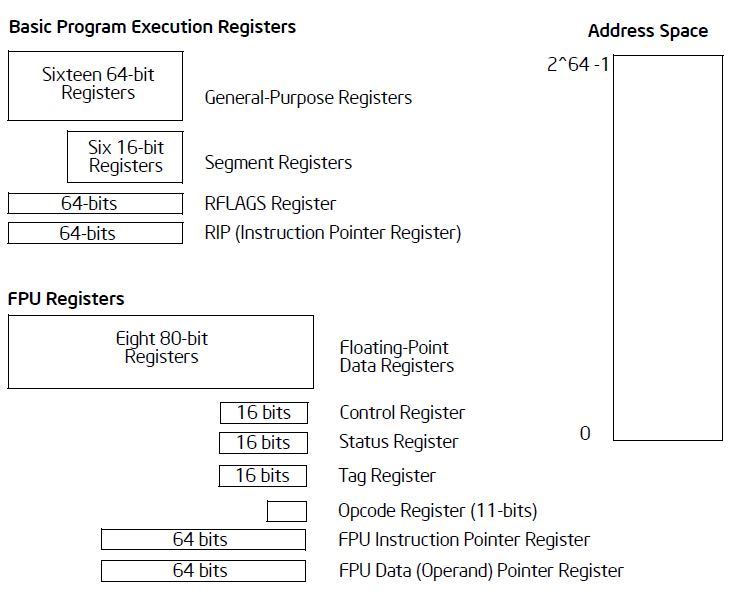
\includegraphics[width=0.8\textwidth]{x86_ovl.JPG}
\end{center}

%pg.29
\subsection{DEC Alpha}
Alpha architecture is a 64-bit load/store RISC architecture developed by
Digital Equipment Corportaion (DEC). The architecture is desinged to be 
a true high speed 64-bit architecture with emphasis on the clock speed, 
multiple instruction issue, and multiple processors. All of the Alpha 
registers are 64-bits width with 32-bit length instructions. 
\par
The
basic addressable unit in Alpha is 8-bit byte, a word is 2 contiguous bytes 
(16 bits), a longword is 4 continuous bytes (32 bits), a quadword
is 8 contigous bytes (64 bits). A virtual address in Alpha are referred
as a 64-bit long quardword. 
\par
In term of floating point number, Alpha supports two floating point standard
(IEEE and VAX standard) with three formats for VAX (F\_floating - 4 bytes, 
G\_float - 8 bytes high-low, D\_float - 8 bytes high-mid-low) and two formats
for IEEE (T\_float - 8 bytes, and X\_float - 16 bytes).


\section{Architecture History}
In this section of the repor, the development history of \textbf{x86} and
\textbf{DEC Alpha} will be discussed. The discussion will be perceived in 
the chronical order.  Along the timeline, there will be a brief discussion
on an architecture modification and its impact on the proceeding 
generations. 

\subsection{IA-32 (x86)}
In 1972, Intel realeased the 8080, their first 8-bit microprocessor.  The
microcontroller was using Datapoint Corporation instruction set with 
programmable CRT terminal. Four years later, Intel had an idea to improve
8085 making the design less-delayed with either 16/32-bit processors.
The design was started with a processor design, namely, 8086  
which upon released (1978) became the first x86 microprocessors. 
As it turn out, the processors were a massive success on both as a physical
chip design and processor architecture. Intel 8086 was unique for its full 
support on 16-bit processing as well as the signed integers, base+offset 
addressing, and self-repeating operations. Later Intel released its cousin
Intel 8088, an Intel 8086 with 16-bit external data bus. 
\sout{\textbf{Remark:} Intel 8088 uses two 8-bit cycle to operate its 
external data bus}
\par
In the 80s, Intel 8088 processor obtained its legacy as a standard processor
for a personal computer thanked IBM 5150, the first personal computer.
At the time, IBM decided to exploit a new market opportunity -- a personal 
computer market. They decided their PC module (5510) should run a 16-bit 
processor and Intel 8088 seemed to be the best candidate due to the 
lowest manufacturing cost with a minimal chip count. On release, the IBM 5150
became one of the most influential PC of all time and Intel 8086 architecture 
got its name as an architecture used in a personal computer.  
\textbf{Note:} x86 architecture lended its name from the legacy 8088 that has
8086 architecture.
\par
Since x86 was released, Intel had been working on adding new features to the
architecture. 
\begin{center}
   \begin{longtable}{l l p{10cm}}
      \textbf{Year} & \textbf{Model}      & \textbf{Features}\\ \hline

      1987 & 8086/8088  & 16-bit processing, Segmentation, Signed integers \\ 
      \hline
      1982 & Intel 286  & Segment limit checking, Read-only/Execute-only 
      			  segment options, Four privileg levels \\
      \hline
      1985 & Intel 386  & 32-bit address bus (up to 4GB of physical memory),
      			  \newline
      			  Segmented-memory model and flat memory model,
			  \newline
			  Paging (fixed 4KB page size for logical
			  memory management), 
			  \newline
			  Support for parallel stages \\
      \hline
      1989 & Intel 486  & Five pipeline stages for instruction decode and
      			  execution units, 
			  \newline
			  8KB on-chip L1 instruction cache, 
			  \newline
			  Integrated x87 FPU,
		          \newline
			  Power saving and system management capabilities\\
      \hline
      1993 & Intel Pentium & Second execution pipeline for superscalar performance,
      			  \newline
      			  (u and v pipelines),
			  \newline
			  Double L1 cache size 16KB total: 8KB intsruction, 
			  8KB data,
			  \newline
			  Use MESI protocol for cache's write-back,
			  \newline
			  Extended paging: allowing both 4MB and 4KB page size,
			  \newline
			  An APIC support for multiple processors,
			  \newline
			  Branch prediction\\
     \hline
     1995\newline-1999 & Intel P6s & Complete execution of retire three instruction 
     			  per clock cycle, 
			  \newline
			  Out-of-order execution,
			  \newline
			  Double L1 cache size 32KB total: 16KB instruction, 
			  16KB data,
			  \newline
			  L2 cache support cache size of 256K, 512K, 1M,
			  \newline
			  Low power stages,
			  Streaming SIMD Extensions (SSE)\\
     \hline
     2000\newline-2006 & Intel Pentium 4 & Intel NetBurst,
			  Pentium 4 hyper-threading,
			  SSE2, SSE3, Intel VT \\
     \hline
   \end{longtable}
\end{center}

\subsection{DEC Alpha}
\indent Back in the 80s, Digital Equipment Corportaion (DEC) had been preeminent
in the microprocessing unit market with PDP11 and VAX.  In 90s, the VAX
became obsolete due to its unscalability and the difficulties 
integrating VAX with pipelining system. Digital Equipment Corportaion 
moved along from the VAX, they introduced a MicroVAX that used VAX 
instruction. In 1992, the Alpha 21064 was introduced. It was the first 
Alpha processor and the most powerful microprocessor in the market at the
time. Architecturally, Alpha 21064 was a lot different from the preceeding 
DEC microprocessors. Alpha 21064 was a RISC based architecture while VAXs
are CISC based. 
\par
Even if Alpha processor was a well designed microprocessor, DEC did not 
have the resources to mass produce and compete with Intel and AMD in the 
processor market; the Alpha processor had never been very popular. Only
about 500,000 Alpha-based server were sold till 2000. Due to the small 
number of customers, the cost base to produce Alpha based system increased
which caused the positive feedback cycle between the number of customers 
and the production cost.
\par
In 1998, DEC decided to sell the company that was barely making any profit 
to Compaq which itself is then acquired by HP in 2002. 
\textbf{Note:} Even though, the Alpha platform is fadding out it still 
consider one of the best server platform every existed. 

\begin{center}
   \begin{longtable}{l l p{10cm}}
      \textbf{Year} & \textbf{Model}      & \textbf{Features}\\ \hline

      1993 & Alpha 21064\newline(EV4S)  & Dynamic branch prediction,
      					  \newline
      					  32-entry fully associative lookaside buffer,
					  \newline
					  5 stages instruction pipeline,
				          \newline
					  32 64-bit register for floating point values,
					  \newline
					  16KB on-die caches (D-cache): 8KB Data, 
					  8KB instruction,
					  \newline
					  128KB to 16MB external secondary cache(S-cahce) supported,
					  \newline
					  34-bit address bus\\

      \hline
      1995 & Alpha 21164\newline(EV5)   & 4 instruction per clock cycle: 2 int, 2 float operations,
      					  \newline
					  Dual-ported D-cache,
					  \newline
					  96KB on-die secondary cache (S-cache),
					  \newline
					  300MHz internal clock (with /2 pre-scaling)\\
      \hline
      1996 & Alpha 21264\newline(EV6)   & Out-of-order execution (up to 20 int and 15 float can be
      					  queueing at once), 
					  \newline
					  Ebox for executing interger instructions: 32 architectural register,
					  \newline
					  40 rename register, 8 PALshadow registers,
					  \newline
					  Fbox for executing floating point instructions (2 float pipelines),
					  \newline
					  Two level on-die caches: D-cache, B-cache,
					  \newline
					  Better branch prediction\\
      \hline
      1998& Alpha 21364\newline(EV7)   &  Double cache size 32KB: 16 D-cache, 16 S-cache,
      					  \newline
					  7-way set associative S-cache (up to 16GB/s at 1.0 GHz),
					  \newline
					  R-box for network router, Using NUMA for multiprocessing system,
					  \newline
					  Inter-architecture fault tolerance (MIPS to Alpha)\\
      \hline
   \end{longtable}
\end{center}

\textbf{Chapter Remark:}
Regardless of how well an architecture is desinged, it is always the customer
and the market demand that keeps the company and the architecture going. 
A well designed architecture would help a company getting a customer
easier but it is not a gaurunteed that a company will be able to keep 
producing the chip. It is all about the market being in the market  at the 
right place at the right time.


\section{System Registers}
This section will be focusing on IA-32 and DEC Alpha on how they manage
their registers in response to the different needs of the different data types.
%-------------------------------------------------------Prog REG
\subsection{Instruction Pointer Register}

%p.80
\subsubsection{IA-32: Instruction Pointer}
The Instruction Pointer (EIP) Register has the offset of the current code segment
for the next instruction. The EIP register cannot be directly read but is 
accessible from software by calling jump or return instructions. The only way 
to read from the EIP is to use CALL instruction and read the returning value
of from the stack.

%p.45
\subsubsection{DEC Alpha: Program Counter}
Program Counter Register (PC) is a register that stores an address of the next 
instruction. The Program Counter register is a 64-bit width register but only
use 62-bits (bit 63-2) -- the first two bits are ignored. The PC register is
not accessible as an integer register but can be manipulated using 
conditional branch or subroutine jump instructions (software).

\subsubsection{Analysis}
By looking at the developer's manual, IA-32 and DEC Alpha use the same concept  
designing the next instruction pointer register -- a register that tells the
program where to go next. Though, there is a minor different on 
what value being stored. In IA-32, the instruction segment offset is
being stored in EIP. In DEC Alpha, the actual address of the next instruction
is being stored. 


%-------------------------------------------------------INT   REG
%x86 cntr timer + int = int reg Alpha
\subsection{Integer Registers}

%p.73
\subsubsection{IA-32: General Purpose Register}

Intel x86 architecture, there are 8 32-bit general purpose registers, and 
6 16-bit segment registers. The registers are named EAX, EBX, ECX, EDX, ESI, 
EDI, EBP, and ESP. They hold operand values for logical and arithmetic 
operations, memeory pointers, or operands for address calculation. Even though
they are general-purpose register, there are some precautions a user should 
keep in mind e.g. ESI is a stack pointer and should not be used for other 
purposes, some x86 instructions require operand contents to be loaded/read
into/from a certain register and should not be overwritten. Typically, each
of the general purpose register has a certain special functionality ties to it.

%TODO: include firgure 3-5 alternate gneral register purpose
\begin{center}
   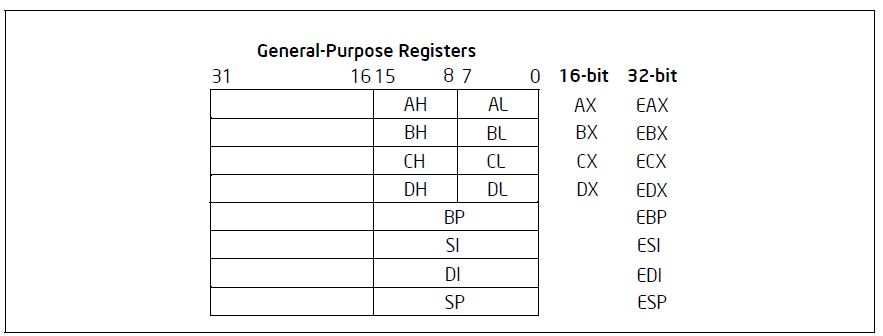
\includegraphics[width=0.8\textwidth]{x86_gen_reg.JPG}

   \begin{longtable}{l p{10cm}}
      \textbf{Register} & \textbf{Special Functionality} \\ \hline
      EAX & Accumulator for operands and results data\\
      EBX & Pointer to data in the DS segment\\
      ECX & Counter for String and loop operations\\
      EDX & I/O pointer\\
      ESI & Source segment offset (the segment location specifies in DS) \\
      EDI & Destination segment offset (the segment location specifies in ES)\\
      ESP & Stack pointer (SS segment)\\
      EBP & Stack offset (SS segment)\\
      \hline
   \end{longtable}
\end{center}


%p.45
\subsubsection{DEC Alpha: Integer Register}
In DEC Alpha architecture, there are 32 64-bit integer registers. They are use
to handle integer operations. Register R31 is reserved and can only be used as 
a source operand with the value of NULL. An instruction that specifies R31 as 
a destination operand are discarded and no signal is issued signifying the 
occurance. It is unpredictable if the destination operands are changed by
the instruction. \textbf{Warning: Do NOT write to R31, bad things will happen}

\subsubsection{Analysis}
From the design, it appears that Intel makes IA-32 integer registers more 
discrete for a specific case of use. While DEC makes their integer registers 
more generic for different purpose uses. In terms of number of the registers,
DEC Alpha outnumbers IA-32 by the magnitude of 4. Although, it is justified
for Intel to have fewer registers in each module (feature) but have a lot more
features for each specific use case.


%-------------------------------------------------------FLOAT REG
\subsection{Floating Points Register}
%p.189
\subsubsection{IA-32: FPU x87 Registers}
In IA-32, Intel uses x87 FPU to handle floating point operations. The
execution environment has eight type of data registers: status, control,
tag word, last instruction pointer, last data (operand) pointer, and opcode.

%TODO: FPU Data Reg stack goes here (firgure8-2)
\begin{center}
   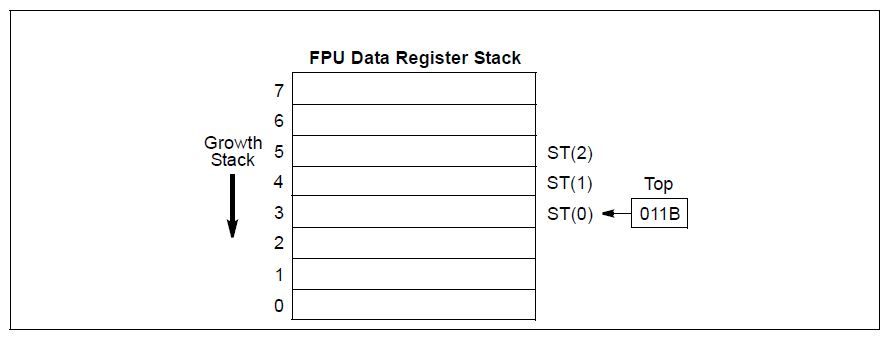
\includegraphics[width=0.8\textwidth]{x86_fpu_stk.JPG}
\end{center}

\par
\textbf{FPU Data Register} has eight 80-bit registers containing anything
from floating point to extended double precision. Any integer values that are
loaded into this register will automatically cast into a floating point 
format. The FPU data register has a stack behavior. Every time a number is
loaded into a register, it will be stored on top of the FPU data stack. 
\textbf{FPU Status Regiser} indicates the currecnt state of the FPU anything
from where is the top of the stack to comparison result to status flags.  
The content of the register can be stored in memory using the floating point
instructions. \textbf{Control Word Register} is where the configuration for 
FPU is stored i.e rounding rules, precision control, etc. \textbf{Infinity
Control Flag Register} is provided to facilitate Intel 287 Math Coprocessor. 
The register does not serve any functionality by itself. \textbf{FPU Tag Word}
indicates the contents of each the 8 registers whether they are valid, zero or 
a special float number (NaN, Inf, denormal, unsupported, or empty). \textbf{Last 
Operand Pointers} stores the pointers to the instruction and data for the last
non-control instruciton executed. \textbf{Last Instruction Opcode} stores in 
11-bit FPU opcode register. 

%P.24, 131
\subsubsection{DEC Alpha: Floating Point Registers}
DEC Alpha architecture uses 32 64-bit \textbf{Floating-Point Registers} to handle its 
double/floating point, register F0 to F31. F31 typically a reserved null register
and holds value of zero when read, the write to F31 are ignored. All 
of the floating point manipulation can be done only between floating point 
registers. The DEC Alpha supports up to maximum of three operands
(two source operands and one destination operand) and can handle 
two different floating point formats (IEEE and VAX floating point). 
Though, during the value manipulation both operands need to be in the same
floating point format. Asides from the data register, DEC Alpha has a \textbf{Floating-Point 
Control Regiser (FPCR)} which is a status and configuration register that would
tell the status of the system and error message of a floating point operation (if any).
\par
\subsubsection{Analysis}
It seems like Intel has a separated, duplicated set of registers specifically 
for handling the floating point numbers and the operations. The set of 
registers are named FPU. FPU has pretty every thing from its own stack 
management to a status register to configuration registers. On the other hand,
DEC Alpha has designated floating point registers that is more integrated with 
the rest of the chip. Although, from a macro perspective, it may look like 
x86 and Alpha architecture are fundamentally different which, of course, they are.
But at the microscopic level, there are some similarity. For an exmaple, 
x86 has FPU Data Registers and DEC Alpha has Floating-Point Registers. Both
of them are the special place where the system put the floating point value 
togehter and do the operation within the register section. Another similarity 
is in the status control registers. In x86, there are Status Register and 
Control Register. Combinding those two registers togehter and that is pretty much
Alpha's Floating-Point Control Register.



%%%%%%%%%%%%%%%%%%%%%%%%%%%%%%%%%%%%%%%%%%%%%%%%%%%%%% END OF SYSTEM REG

\section{Instruction Formats}
In this section of the paper, the concept of instruction formats  will be
discussed. Given the instruction formats of IA-32 and DEC Alpha are drastically 
different in term of design fundamental -- one is functional-oriented, the other is
byte pattern oriented. For the sake of paper's simplicity, the section will be divided 
into two subsections: IA-32 instruction formats and DEC Alpha instruction formats. 
%pg.479 ch 2.1 vol 2
\subsection{IA-32 Instruction Formats}
IA-32 instruction comprises of 6 different parts: prefix, primary opcod, addressing-form
specifier (ModR/M and SIB), displacement and immediate data field. 

%Insert the x86 Instr format layout
\begin{center}
   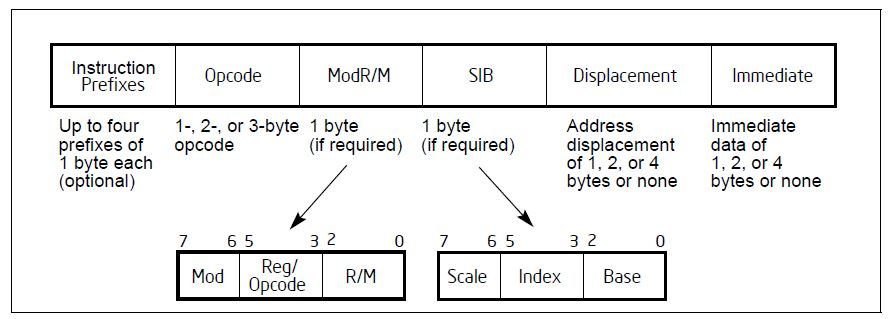
\includegraphics[width=0.8\textwidth]{x86_instr_format.JPG}
\end{center}

\textbf{Instruction Prefix} is the first section of Intel IA-32 instruction. 
It signifies how should the rest of the instruction be interpreted. Prefixes can be 
categorized into four different groups: Lock and Repeat prefixes, Branch Hints, Bound
prefix, Operand-size Override prefix, and Address-size prefix. Lock prefix 
forces an operation to ensure the exclusivity of the shared memory in a multiprocessing 
environment. Repeat prefix forces an instruction to be repeated for each element
of a string. Branch Hints allows a program to guess the code path for a branch.
Address-size Override prefix allows a program to switch between 16 and 32-bit 
operations. \textbf{Opcodes} typically, IA-32 opcode has the size of 1 to 3 bytes with
the last 3-bit embedded in the ModR/M bytes. \textbf{ModR/M Bytes} are the 
opcode modifiers. They play a very crutial role in translating the opcode between mode
of operations -- it provides x86 with a dynamic opcode scheme. In some cases, ModR/M
requires an extra scaling parameters, the parameters can be found in \textbf{the SIB 
bytes}. Some addressing forms include an offest for the ModR/M bytes, the offset can be 
found in \textbf{Displacment and Immediate Bytes}. 

%pg.50 ch.3
\subsection{DEC Alpha Instruction formats}
DEC Alpha instruction format is design to be functionally efficient. 
An instruction is designed to be self-contained and have only a specific use case.
The instruction for DEC Alpha system can be divided into 5 different categories:
memory, branch, operation, floating point operation, and PALcode

%TODO: Insert the DEC Alpha Instruion format layout
\begin{center}
   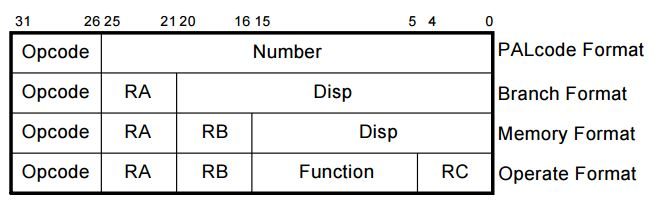
\includegraphics[width=0.6\textwidth]{instr_format_alp.JPG}
\end{center}


\textbf{Memory instruction format} is used to transfer data between memory register,
to loade an effective address, and for subroutine jumps. Typically, the instruction 
contains four parts: opcode, source operands, destination operands, and displacement
(or function field). \textbf{Branch Instruction} is used when conditional branching 
and jumping subroutine is called. The instruction only has 3 components: opcode, 
an operand, and branch displacement. The branch displacment is a sign-extended 64-bit
ready to up date the PC value. \textbf{Operation Instruction} is used for an instruction
that perform integer register to integer register operations. The operation format allows
one destination operand and up to two source operands. \textbf{Floating Point Operation
Instruction} is used to perform float on float operations. The format allows one 
destination operand and up to two source operands. \textbf{PALcode Instruction} is used
to specify extended processor functions. 

%TODO: insert DEC float and int oper format

\subsection{Analysis}
IA-32 instruction is design to be more byte pattern oriented. 
By looking at the byte pattern, a user can tell exactly the system mode of operation,
location of the operands, and the function that is being executed. 
The design is necessary for x86 architecture because x86 has multiple mode of operations
and each mode takes a different format of the opcode. To facilitate the needs, a dynamic
opcode scheme is required. On the other hand, DEC Alpha instructions are designed to be
work with a high performance architecture; there needs to be minimal instruction overhead 
either from translation or accessing value from a different register. That is why the 
DEC Alpha instructions are concise and self-contained.





\newpage
\nocite{*}
\bibliographystyle{IEEEannot}
\bibliography{ECE472_sawaspar_final_paper}
\end{document}
